\section{Sezione Utente}
\label{sec:sezUtente}

\subsection{Visualizzazione mobile}
\begin{figure}[H]
  \centering
  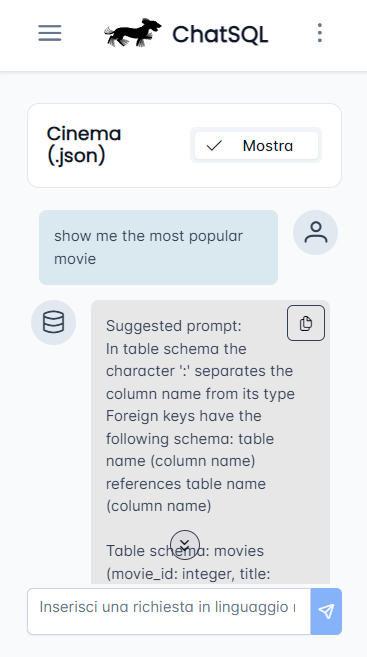
\includegraphics[width=0.50\textwidth]{assets/mobile.png}
  \caption{Versione mobile dell'applicazione}
\end{figure}
\par L'applicazione è stata progettata per essere fruibile anche da dispositivi mobili per garantire una buona esperienza d'uso con schermi touch screen di piccole dimensioni.  
\par Per migliorare la navigazione da dispositivi mobili, il menù principale, di default è nascosto e può essere aperto cliccando l'icona a tre linee 
\includegraphics[height=1.2em]{assets/dd_burger_menu.png} in alto a sinistra.
\par Le viste dell'applicazione occupano tutta la grandezza dello schermo, per dare più spazio possibile al contenuto principale.
\par Per ridurre l'ingombro dello schermo, i bottoni di login e delle impostazioni di sistema, sono accessibili mostrando un menù a tendina, cliccando sull'icona a tre puntini 
\includegraphics[height=1.2em]{assets/dd_kebab_menu.png} in alto a destra.

\subsection{Impostazioni di sistema}
Nella sezione superiore destra dell'interfaccia, cliccando sull'icona impostazioni 
\includegraphics[height=1.2em]{assets/settings_icon.png}, apparirà il menu laterale delle impostazioni di sistema.
\begin{figure}[H]
  \centering
  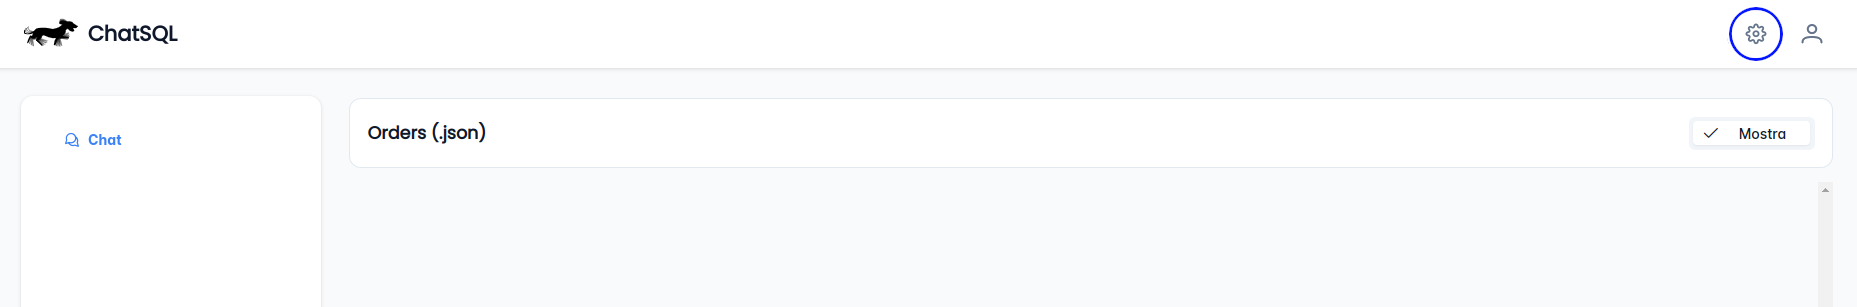
\includegraphics[width=1\textwidth]{assets/settings_topbar.png}
  \caption{Topbar con icona delle impostazioni}
\end{figure}
\begin{figure}[H]
  \centering
  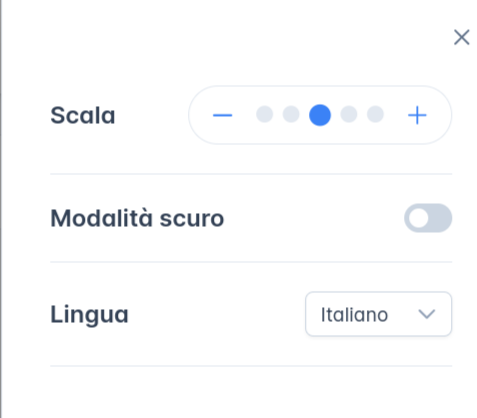
\includegraphics[width=0.50\textwidth]{assets/menu_config.png}
  \caption{Menu laterale delle impostazioni di sistema}
\end{figure}
\par Le impostazioni di sistema permettono di configurare le seguenti opzioni:
\begin{itemize}
  \item Scala: dimensioni del testo e della schermata; utile per adattare la dimensione dell'interfaccia alle proprie esigenze;
  \item Tema scuro: abilita o disabilita il tema scuro dell'interfaccia, per personalizzazione, accessibilità e comfort visivo;
  \item Lingua: selezione della lingua dell'interfaccia tra inglese e italiano (non cambia la lingua del \glossario{prompt} prodotto da ChatSQL, che rimane sempre in inglese).
\end{itemize}
\par Le modifiche apportate verranno memorizzate automaticamente, e applicate alla successiva apertura dell'applicazione.

\subsection{Workflow}
\par Nell'utilizzo di ChatSQL, il flusso più comune da seguire per ottenere una query SQL è:
\begin{enumerate}
  \item Entrare nella pagina Chat selezionandola dal menu principale;
  \item Selezionare il dizionario dati desiderato;
  \item Selezionare il DBMS desiderato;
  \item Inserire la richiesta in linguaggio naturale e attendere la generazione del prompt;
  \item Copiare il prompt generato cliccando sul bottone in alto a destra sul messaggio prodotto da ChatSQL;
  \item Incollare il prompt in un modello LLM a scelta (come ChatGPT) e attendere la generazione della query SQL.
\end{enumerate}
TODO: aggiungere immagini per ogni punto
\par L'output atteso dal modello LLM è una query SQL che soddisfa la richiesta inserita, che potrà essere eseguita su un DBMS per ottenere i risultati desiderati.